\documentclass[a4paper]{article}
\usepackage{amsmath, amssymb, amsfonts}
\usepackage[margin=1in]{geometry}
\usepackage{graphicx}
\usepackage{tikz}
\usepackage{esint}
\setlength{\parindent}{0em}
\setlength{\parskip}{1ex}
\newcommand{\vct}[1]{\overrightarrow{#1}}
\newcommand{\dif}{\mathrm{d}}
\newcommand{\pd}[2]{\frac{\partial {#1}}{\partial {#2}}}
\newcommand{\dd}[2]{\frac{\mathrm{d} {#1}}{\mathrm{d} {#2}}}
\newcommand{\C}{\mathbb{C}}
\newcommand{\R}{\mathbb{R}}
\newcommand{\Q}{\mathbb{Q}}
\newcommand{\Z}{\mathbb{Z}}
\newcommand{\N}{\mathbb{N}}
\newcommand{\fn}[3]{{#1}\colon {#2} \rightarrow {#3}}
\newcommand{\avg}[1]{\langle {#1} \rangle}
\newcommand{\Sum}[2][0]{\sum_{{#2} = {#1}}^{\infty}}
\newcommand{\Lim}[1]{\lim_{{#1} \rightarrow \infty}}
\newcommand{\Binom}[2]{\begin{pmatrix} {#1} \cr {#2} \end{pmatrix}}

\begin{document}
\paragraph{Gibanje telesa v sferičnem potencialu.} $$E = \frac{1}{2}m\dot{r}^2 + V_{ef}(r)$$
Tu je $\displaystyle{V_{ef} = V(r) + \frac{l^2}{2mr^2}}$ in $l = mr^2\dot{\varphi}$. Zdaj lahko izrazimo $\dot{r}$ kot
$$\dd{r}{t}=\pm\sqrt{\frac{2}{m}}\left(E - V_{ef}(r)\right)^{1/2}$$
$$\int_{t_0}^{t_1}\dif t = \pm\sqrt{\frac{m}{2}}\int_{r_0}^{r(t_1)}\frac{\dif r}{\sqrt{E - V_{ef}(r)}}$$
$$\dd{r}{t} = \dd{r}{\varphi}\dd{\varphi}{t}$$
Sledi:
$$\varphi = \pm \sqrt{\frac{1}{2m}} \int_{r_0}^{r(t)} \frac{l\dif r}{r^2\sqrt{E - V_{ef}(r)}}$$
Iz $\varphi(r)$ pa lahko dobimo $r(\varphi)$.
\paragraph{Klasifikacija orbit.} Za Keplerjev potencial smo to storili že na vajah. Zdaj obravnavajmo potencial $\displaystyle{V = -\frac{|\alpha|}{r^\beta}}$ \\[2mm]
$\beta < 2$: $\displaystyle{\frac{l^2}{2mr^2} > \left|\frac{\alpha}{r^\beta}\right|}$, podobno kot pri Keplerju. \\[2mm]
$\beta = 2$: Cotesova vijačnica (zelo lahko rešimo, celo lažje, kot s Keplerjevim potencialom.) \\[2mm]
$\beta > 2$: Efektivni potencial bo izgledal približno takole:
\begin{figure}[h!]
    \includegraphics{Screenshot_20250409_105100.png}
\end{figure}
\\[2mm]
Splošno: $V(r) = |\alpha|r^\beta$,
Če je $\beta = -2, -1, 1$, lahko stvar opišemo s trigonometričnimi funkcijami. Če je $\beta = -6, -4, -3, 1, 4, 6$, dobimo eliptične integrale. Sicer je problem rešljiv numerično ali pa celo ni rešljiv.
\paragraph{Problem treh teles.} Ni analitično rešljiv. Rešujemo pa ga lahko numerično.
\paragraph{Lagrangeova točka.} Če se postavimo med Zemljo in Sonce, bo na nas delovala tako privlačna sila Zemlje kot privlačna sila Sonca. Prva Lagrangeova točka je med Zemljo in Soncem, tako da je vsota gravitacijskih privlakov enaka 0. Druga Lagrangeova točka je na zunanji strani Zemljive orbite (razno tako v taki točki, da imata Zemlja in Sonce enak privlak).
Tretja je na nasprotni strani Sonca glede na Zemljo, četrta in peta pa sta iz premice, ki povezuje Zemljo in Sonce, izmaknjeni za približno $60^\circ$.
\paragraph{Zanimivost:} V četrti in peti Lagrangeovi točki Jupitra se je skozi čas nabralo večje število asteroidov. Lagrangeove točke predstavljajo ene izmed stabilnih rešitev problema treh teles.
\paragraph{Teorija kaosa.} Če se začetni pogoji že zelo malo razlikujejo, bosta gibanji po dovolj dolgem času zelo različni.
To pomeni, da problem treh teles sicer lahko rešujemo numerično, vendar se bodo numerične napake zelo poznale.
\paragraph{Gibanje togega telesa.} Najprej moramo telo dobro opisati.
\paragraph{Eulerjevi koti.} Poskusimo opisati rotacijo v ravnini. Ločimo več oblik rotacij. \\[2mm]
Pasivna rotacija:
\begin{figure}[h!]
    \centering
    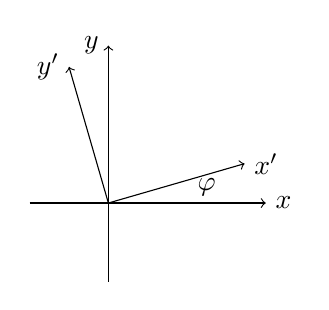
\begin{tikzpicture}
        \draw[->] (-1, 0) -- (2, 0) node[right] {$x$};
        \draw[->] (0, -1) -- (0, 2) node[left] {$y$};
        \draw[->] (0, 0) -- (1.73, 0.5) node[right] {$x'$};
        \draw[->] (0, 0) -- (-0.5, 1.73) node[left] {$y'$};
        \node (A) at (1.25, 0.2) {$\varphi$};
    \end{tikzpicture}
\end{figure}
$$\begin{pmatrix}
    \cos\varphi \\ -\sin\varphi \\ z
\end{pmatrix} =
\begin{pmatrix}
    \cos\varphi & \sin\varphi & 0 \\
    -\sin\varphi & \cos\varphi & 0 \\
    0 & 0 & 1
\end{pmatrix} \begin{pmatrix}
    1 \\ 0 \\ z
\end{pmatrix}$$
Oziroma $\vct{r}' = R_{3}(\varphi) \vct{r}$ \\[2mm]
Aktivna rotavija:
$$\begin{pmatrix}
    \cos\varphi \\ \sin\varphi \\ z
\end{pmatrix} =
\begin{pmatrix}
    \cos\varphi & -\sin\varphi & 0 \\
    \sin\varphi & \cos\varphi & 0 \\
    0 & 0 & 1
\end{pmatrix} \begin{pmatrix}
    1 \\ 0 \\ z
\end{pmatrix}$$
Ortogonalna transformacija: Preslikava z lastnostjo $\det R = 1$. Poleg tega mora veljati $R^TR = I$ in
$$\vct{a}'\cdot\vct{b}' = R\vct{a}\cdot R\vct{b} = \vct{a}\cdot\vct{b}$$
\end{document}